\begin{table}[ht]
	\begin{center}
	\resizebox{1.0\columnwidth}{!}{%resize the table
		\begin{tabular}{|l|cc|cc|}
			\hline
			\multirow{2}{*}{Methods}	&  
             \multicolumn{2}{c|}{\textsc{QAMR-SUBSET}}&\multicolumn{2}{c|}{\textsc{PTB-SUBSET}} \\
             \cline{2-5}
           & accuracy & recall  & accuracy & recall  \\

                        \hline
            Gradient Boosting
            & .488 & .501 & .338 & .388  \\
            Gradient Boosting discourse
            & .673 & .681 & .575 & .632  \\
            BM25
            & .536 & .549 & .456 & .528  \\
            Xgboost Rank
            & .469 & .481 & .360 & .431  \\
            Xgboost Rank
            & .670 & .678 & .561 & .618  \\
            BoW
            & .540 & .549 & .405 & .458  \\
            CNN
            & .511 & .521 & .387 & .430  \\
            \hline
            DRMbinary discourse
            & .664 & .672 & .573 & .637  \\
            DRM
            & .702 & .724 & .599 & .676  \\
            DRMhuman
            & .767 & .779 & .663 & .714  \\
            \hline

		\end{tabular}
		}
	\end{center}
	\caption{Comparison of different approaches. ``-'' means result not available.
    }\label{tab:main}
\end{table}


\begin{figure}[t]
	{\fontsize{9}{10}\selectfont
    \setlength{\tabcolsep}{0.6mm}
%    \hspace{-2mm}
    \begin{tabular}{|p{75mm}|}
    \hline
\textbf{Context: }Given its initial condition, prediction of its final condition is possible, causally \textcolor{red}{but} only probabilistically, \textcolor{red}{because} the Schrödinger equation is deterministic for wave function evolution, \textcolor{red}{but} the wave function describes the system only \textcolor{blue}{probabilistically}.\\
\textbf{Question: }Why is the prediction
\textcolor{blue}{probabilistic}? \\
(\textit{reasoning step 1: find the word because for why-question and read the left side of it.})\\
\textbf{Context: }the Schrödinger equation is deterministic for wave function evolution, \textcolor{red}{but} the wave function describes the system only \textcolor{blue}{probabilistically}.\\
(\textit{reasoning step 2: find the word but and read the left side of it})\\
\textbf{Answer: }the wave function describes the system only probabilistically\\
\hline
    \end{tabular}
    }
\caption{Example QAMR: We highlight discourse marker in read and target words in blue. blabla \cheng{Don't just use colors}}
\label{fig:qa_example_reason}
\end{figure}



\begin{table*}[ht]
	\begin{center}
	\resizebox{2.0\columnwidth}{!}{%resize the table
		\begin{tabular}{|l|cc|cccccccc|}
			\hline
             method
           & accuracy & recall  & what & whose & how & why & where & who & when & which  \\

                        \hline
            Gradient Boosting
            & .488 & .501 & .485 & .523 & .502 & .461 & .477 & .471 & .517 & .561  \\
            Gradient Boosting discourse
            & .673 & .681 & .676 & .633 & .664 & .538 & .659 & .662 & .721 & .684  \\
            BM25
            & .536 & .549 & .545 & \textbf{.679} & .543 & .160 & .529 & .510 & .464 & .594  \\
            Xgboost Rank
            & .469 & .481 & .486 & .397 & .414 & .566 & .475 & .447 & .453 & .457  \\
            Xgboost Rank discourse
            & .670 & .678 & .673 & .638 & .657 & .538 & .657 & .662 & .721 & .684  \\
            BoW
            & .540 & .549 & .539 & .490 & .506 & .615 & .524 & .552 & .571 & .558  \\
            CNN
            & .511 & .521 & .508 & .528 & .515 & .564 & .496 & .513 & .517 & .522  \\
            \hline
            DRMbinary discourse
            & .664 & .672 & .667 & .619 & .649 & .564 & .653 & .657 & .706 & .678  \\
            DRMtype1
            & .691 & .711 & .696 & .676 & .681 & .615 & .696 & .671 & .724 & .702  \\
            DRMtype2
            & \textbf{.702} & \textbf{.724} & \textbf{.703} & .676 & \textbf{.684} & \textbf{.615} & \textbf{.701} & \textbf{.677} & \textbf{.733} & \textbf{.705}  \\
            DRMhuman
            & \textbf{.767} & \textbf{.779} & \textbf{.767} & \textbf{.757} & \textbf{.761} & \textbf{.717} & \textbf{.765} & \textbf{.767} & \textbf{.795} & \textbf{.759}  \\
            \hline

		\end{tabular}

		}\vspace{0.5cm}
\resizebox{2.0\columnwidth}{!}{%resize the table
		\begin{tabular}{|l|cc|cccccccc|}
			\hline
             method
           & accuracy & recall  & what & whose & how & why & where & who & when & which  \\

                        \hline
            Gradient Boosting
            & .338 & .388 & .355 & .363 & .289 & .166 & .291 & .311 & .263 & .428  \\
            Gradient Boosting discourse
            & .575 & .632 & .586 & .528 & .616 & .666 & .632 & .621 & .610 & .528  \\
            BM25
            & .456 & .528 & .481 & .380 & .393 & .0.0 & .448 & .439 & .444 & .491  \\
            Xgboost Rank
            & .360 & .431 & .376 & .454 & .339 & .666 & .354 & .335 & .276 & .301  \\
            Xgboost Rank discourse
            & .561 & .618 & .567 & .424 & .578 & .166 & .583 & .566 & .539 & .507  \\
            Chunked BoW Model
            & .405 & .458 & .422 & .363 & .408 & .166 & .312 & .376 & .315 & .492  \\
            CNN
            & . & . & . & . & . & . & . & . & . & .  \\
            \hline
            DRMbinary discourse
            & .573 & .637 & .571 & .606 & .591 & .833 & .645 & .572 & .513 & .539  \\
            DRMtype1
            & . & . & . & . & . & . & . & . & . & .  \\
            DRMtype2
            & .599 & .676 & .599 & .575 & .616 & .833 & .666 & .598 & .565 & .523  \\
            DRMhuman
            & .663 & .714 & .665 & .606 & .702 & .833 & .562 & .677 & .578 & .650  \\
            \hline

		\end{tabular}

		}\vspace{0.5cm}		
	\resizebox{2.0\columnwidth}{!}{%resize the table
		\begin{tabular}{|l|cc|cccccccc|}
			\hline
             method
           & accuracy & recall  & what & whose & how & why & where & who & when & which  \\

                \hline
            Gradient Boosting
            & . & . & . & . & . & . & . & . & . & .  \\
            Gradient Boosting discourse
            & . & . & . & . & . & . & . & . & . & .  \\
            BoW
            & .367 & .420  & .369 & .272 & .402 & .333 & .250 & .358 & .473 & .317  \\
            DRMtype2
            & .596 & .673 & .601 & .515 & .616 & .833 & .625 & .592 & .565 & .507  \\
            DRMtype2\_ptb
            & .599 & .676 & .599 & .575 & .616 & .833 & .666 & .598 & .565 & .523  \\
            \hline

		\end{tabular}

		}		
	\end{center}
	\caption{Comparison of different approaches.
    }\label{tab:main}
\end{table*}

\begin{table*}[t]
\centering
{
	\fontsize{9}{9}\selectfont
    %\setlength{\baselineskip}{0pt}
    \setlength{\tabcolsep}{1.0mm}
    \renewcommand{\arraystretch}{1.1}
	%\hspace{4mm}
	\begin{tabular}{|c|c|c|}
 	\hline
  	Learned Reasoning & {Sample discourse markers} & Sample QA pairs \\
  	\hline
 	Answer and target word are at the same side & and, then, or, also, without, before, after, because &  \\
    \hline
 	Answer and target word are at different sides & rather, as soon as, yet, at least, because of &\\
 	\hline
\end{tabular}
}
\caption{\fontsize{10}{12}\selectfont Sample discourse markers from our predefined lexicon.}
\label{tab:discourse_markers}
\end{table*}


\begin{figure}
\begin{minipage}{.49\textwidth}
  \centering
  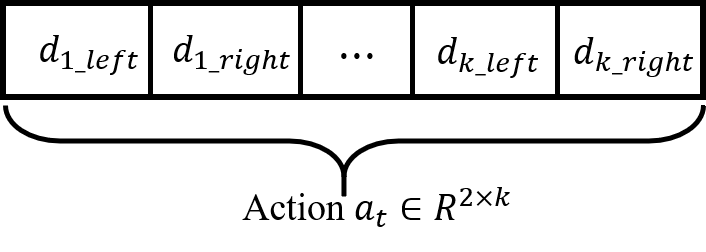
\includegraphics[width=0.9\linewidth]{fig/fig2.png}
  \caption{Type 1 Action}
  \label{fig:type1action}
\end{minipage}
\end{figure}
\begin{figure}
\begin{minipage}{.49\textwidth}
  \centering
  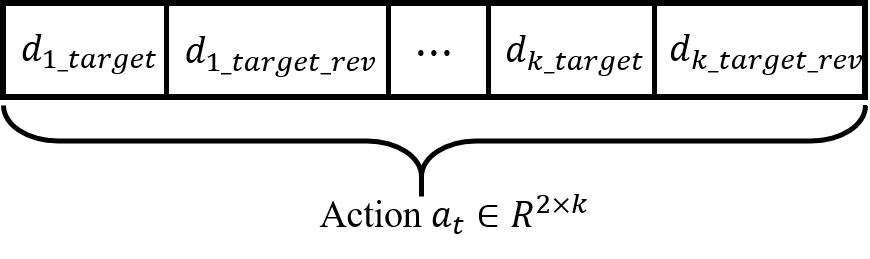
\includegraphics[width=0.9\linewidth]{fig/fig3.png}
  \caption{Type 2 Action}
  \label{fig:type2action}
\end{minipage}
\end{figure}
%These word markers can be in many different forms, like: the frequently used verbs, the target names/dates/locations and the connectives linking clauses or sentences.

\begin{figure}
\begin{minipage}{.49\textwidth}
  \centering
  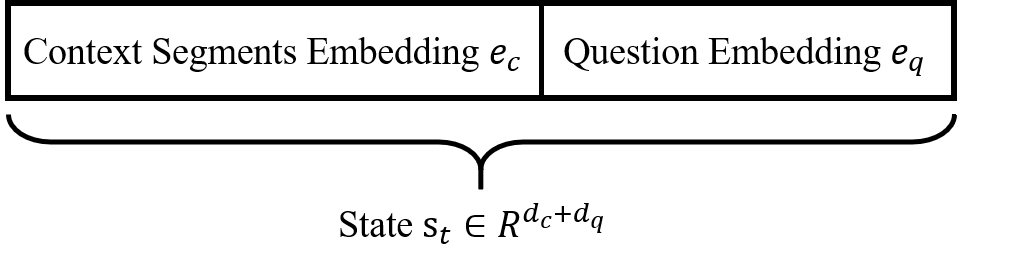
\includegraphics[width=0.9\linewidth]{fig/fig4.png}
  \caption{State Definition}
  \label{fig:state}
\end{minipage}
\end{figure}

\begin{equation}
r=
    \begin{cases}
      1 & \text{if $A^* \subseteq S_{final}$}\\
     0 & \text{otherwise}\\
    \end{cases}
\end{equation}

We compare our methods with the following methods: \\
\textbf{Gradient Boosting}. As a simple baseline, for a given question, we use a binary classifier to evaluate  different (question, segment) pairs and select the segment with the highest prediction score. Bag-of-words features are first extracted separately from both the question and the segment and then concatenated. In order to capture interactions between words in the question and words in the segment, we choose Gradient Boosting~\cite{friedman2001greedy} as the binary classifier since it is very effective in modeling feature interactions. Two variants of Gradient Boosting are tested, one (named GB-binary) trained with binary cross entropy loss, the other (named GB-ranking) with ranking loss. In additional to bag-of-words features, we also considered discourse features, which have been shown to be effective for answering question \cite{DBLP:conf/acl/JansenSC14,DBLP:conf/acl/NarasimhanB15}. We introduce four new discourse features: left discourse marker, right discourse marker, the position of the target word, and the question type.\\
\textbf{BM25} We use BM25~\cite{DBLP:journals/ftir/RobertsonZ09} as a bag-of-words retrieval function to rank segments based on the question terms appearing in each segment.\\
\textbf{Chunked BoW Model}~\cite{DBLP:conf/acl/ChoiHUPLB17}. This is similar to the GB-binary model, except that the binary classifier employed is a neural network with fully connected layers.\\
\textbf{CNN}~\cite{DBLP:conf/acl/ChoiHUPLB17} \cheng{kechen please write}

\begin{itemize}
    \item \textbf{Gradient Boosting}. As a simple baseline, for a given question, we use a binary classifier to evaluate  different (question, segment) pairs and select the segment with the highest prediction score. Bag-of-words features are first extracted separately from both the question and the segment and then concatenated. In order to capture interactions between words in the question and words in the segment, we choose Gradient Boosting~\cite{friedman2001greedy} as the binary classifier since it is very effective in modeling feature interactions. Two variants of Gradient Boosting are tested, one (named GB-binary) trained with binary cross entropy loss, the other (named GB-ranking) with ranking loss. In additional to bag-of-words features, we also considered discourse features, which have been shown to be effective for answering question \cite{DBLP:conf/acl/JansenSC14,DBLP:conf/acl/NarasimhanB15}. We introduce four new discourse features: left discourse marker, right discourse marker, the position of the target word, and the question type.
    \item \textbf{BM25} We use BM25~\cite{DBLP:journals/ftir/RobertsonZ09} as a bag-of-words retrieval function to rank segments based on the question terms appearing in each segment.
    
    \item \textbf{Chunked BoW Model}~\cite{DBLP:conf/acl/ChoiHUPLB17}. This is similar to the GB-binary model, except that the binary classifier employed is a neural network with fully connected layers.
    \item \textbf{CNN}~\cite{DBLP:conf/acl/ChoiHUPLB17} \cheng{kechen please write}
\end{itemize}


We consider the following variants of our method:
\begin{itemize}
\item \textbf{DRM-type 1} Our deep reasoning model with type 1 action, as described in Section 3.2.
\item \textbf{DRM-type 2} Our deep reasoning model with type 2 action, as described in Section 3.2.
\item \textbf{DRM-type 2 w/ human} We consider a variant of our deep reasoning model with human in the loop, in order to demonstrate that our model has the ability to interact with humans. At each decision step, if the algorithm's confidence in its best action is lower than some pre-specified threshold (e.g. 0.5), the algorithm asks a human to help make a decision. We assume that humans always make the right decision w.r.t. the ground truth. 
\end{itemize}

\begin{table}[t]
\centering
\fontsize{9}{10}\selectfont
%\setlength{\baselineskip}{0pt}
\setlength{\tabcolsep}{1.5mm}
\begin{tabular}{|l|c|}
    \hline
%         &\multicolumn{2}{c|}{\textbf{SVM}}\\ 
        & \textbf{Acc} \\ \hline
        \newcite{DBLP:conf/emnlp/StabG14} & 42.2   \\ 
        DRM & 53.3   \\ \hline
\end{tabular}
\caption{\fontsize{10}{12}\selectfont Major claim extraction results on persuasive essay dataset.}
\vspace{-2ex}
\label{tab:majorclaim}
\end{table}




\begin{table*}[t]
\centering
{
	\fontsize{9}{9}\selectfont
  %\setlength{\baselineskip}{0pt}
  \setlength{\tabcolsep}{1.0mm}
  \renewcommand{\arraystretch}{1.1}
	%\hspace{4mm}
	\begin{tabular}{|p{2cm}|p{4cm}|p{1.5cm}|p{1.5cm}|p{6cm}|}
 	\hline
 	\textbf{Question genre} & \textbf{Relevant discourse markers}& \textbf{Same side}& \textbf{Opposite sides} & \textbf{Example QA pairs} \\
 	\hline
 	when \newline what year \newline how long 
 	& \textbf{step 1}: as soon as, at that, previously, until, back, after, soon, yet, such as, last \newline \textbf{step 2}: as soon as, since, second, soon, next, after, when, as well, because, who 
	& already \newline again \newline still \newline following \newline while & as soon as \newline originally \newline then \newline at that \newline further
 	& \textbf{Context: }28 \textit{\textcolor{blue}{skiers}} earned DNFs \textit{\textcolor{red}{during}} \underline{the first run}, \textit{\textcolor{red}{and}} nine earned DNFs \textit{\textcolor{red}{during}} their second runs.
  \newline \textbf{Question: }When did \textit{\textcolor{blue}{skiers}} earn DNFs? 
  \newline \textbf{Learned Reasoning: } during-right, and-left\\ 
	\hline
  why \newline what caused 
  &\textbf{step 1}: in order to, because, at that, previously, though, if, since, still, too, like \newline \textbf{step 2}: following, which, second, for, as, to, or, that, not, and & well \newline initially \newline which \newline even \newline following & in order to \newline since \newline because \newline as \newline but
  & \textbf{Context: }Given its initial condition, prediction of its final condition is possible, causally \textit{\textcolor{red}{but}} only probabilistically, \textit{\textcolor{red}{because}} the Schrödinger equation is deterministic for wave function evolution, \textit{\textcolor{red}{but}} \underline{the wave function describes the system only} \underline{\textit{\textcolor{blue}{probabilistically}}}.
  \newline \textbf{Question: }Why is the prediction \textit{\textcolor{blue}{probabilistic}}?
  \newline \textbf{Learned Reasoning: }because-right, but-right\\ 
	\hline	
	who+past tense 
	&\textbf{step 1}: earlier, ultimately, definitely, since, when, later, while, before, previously, finally \newline \textbf{step 2}: too, yet, second, initially, including, after, next, again, last, and  
	& rather \newline thus \newline including \newline nor \newline who & earlier \newline definitely \newline particularly \newline seemingly \newline previously
	
	& \textbf{Context: }\underline{Hatch had} \textit{\textcolor{red}{previously}} \textit{\textcolor{blue}{survived}} a separate crash in 2003, \textit{\textcolor{red}{that}} killed his mother, brother \textit{\textcolor{red}{and}} sister.
  \newline \textbf{Question: }Who \textit{\textcolor{blue}{survived}}?\newline \textbf{Learned Reasoning: }previously-left\\ 
	\hline
  where 
  & \textbf{step 1}: in which, back, in that, to, then, eventually, second, next, before \newline \textbf{step 2}: too, yet, second, initially, including, after, next, again, last, and
  
	 & following \newline to explain \newline like \newline finally \newline hence & to \newline before \newline eventually \newline back \newline in that
  & \textbf{Context: }\textit{\textcolor{red}{Once}} the proposed \textit{\textcolor{blue}{amendment}} has passed those hurdles, \textit{\textcolor{red}{then}} the amendment goes \textit{\textcolor{red}{to}} \underline{Indiana voters} \textit{\textcolor{red}{who}} vote yea or nay on the amendment. 
  \newline \textbf{Question: }Where does the \textit{\textcolor{blue}{amendment}} go?
  \newline \textbf{Learned Reasoning: }right-to, left-who\\ 
 \hline
\end{tabular}
}
\caption{\fontsize{9}{12}\selectfont Top 10 discourse markers associated with question types and top 5 discourse markers associated with focus direction learned in \textsc{QAMR-SUBSET} dataset. We show four different question genres: time, reason, person, and location.}
\label{tab:disc_phrase}
\vspace{-0.5em}
\end{table*}


(see Table \ref{tab:stats} for stats).
 % We also report the number of text segments segmented by discourse markers and the average number of words in each segment .
\begin{table}[h]
	\resizebox{1.01\columnwidth}{!}{%resize the table
\begin{tabular}{|l|c|c|}
  \hline
   & \textsc{QAMR-SUBSET} & \textsc{PTB-SUBSET}   \\
  \hline
  \# Context Paragraphs in train & 2,706 & 143 \\
  \# Context Paragraphs in test & 329 & 27 \\
  \# QA Pairs in train & 28,918 & 7,941   \\
  \# QA Pairs in test & 10,519 & 1,781  \\
  \# segments/context & 3.58 & 3.54   \\
  \# words/segment & 6.30 & 6.84 \\
  \hline
\end{tabular}
}
\caption{\fontsize{10}{12}\selectfont  Statistics of the datasets.}\label{tab:stats}
%\vspace{-3ex}
\end{table}
%\vspace {-3ex}


\begin{figure}\centering
\begin{minipage}{.45\textwidth}
 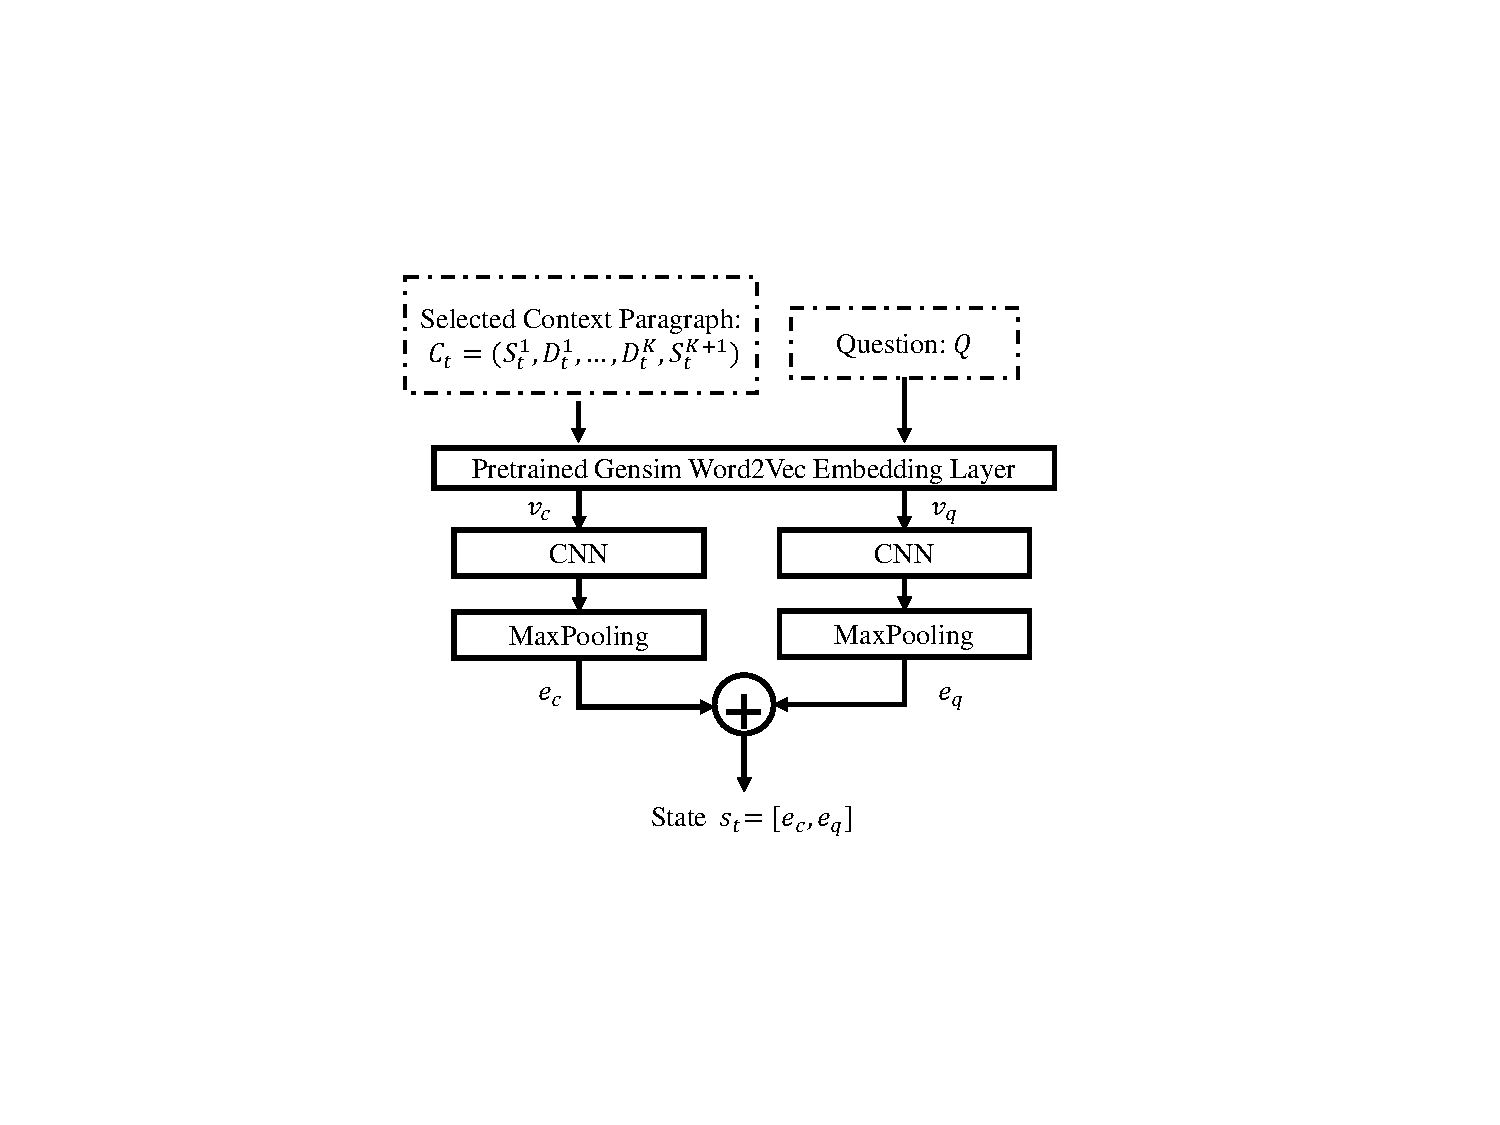
\includegraphics[width=0.9\linewidth]{fig/fig1_2.pdf}
 \caption{SGM Diagram}
 \label{fig:sgmDiagram}
\end{minipage}
\vspace{-2ex}
\end{figure}

To verify our speculation, we simulate coarse-to-fine step by selecting a short text span around the labeled answer. The extracted text spans contain 5.7 discourse markers in average and serve as new context. We then apply our model on it to predict the answer segment. Experimental results show that the overall accuracy on whole SQuAD dev dataset is 0.82. This new result is much better than it on original dataset and comparable to STOA result. 